\section{Theoretical foundations}

This section represents the theoretical fundamentals of this elaboration by defining the term \enquote{data analytic}, the concept of the \enquote{information value chain} and the experimental research process in general.

%\subsection{Definition of terms}

\subsection{Design Science Research Methodology}

In order to accomplish the goal of this thesis, to create an artifact for the improvement of the research process in the field of data analytics, the \ac{dsr} approach the approach is briefly discussed and introduced. In fundamental terms, design science is a research approach that aims to develop and validate science-based design knowledge and guide research to problem solving (\cite{Hevner.2004}, \cite{Dresch.2015}). The goal of \ac{dsr} is to gain prescriptive knowledge about the composition of various artifacts, including software, methods, models, and concepts. This particular design knowledge facilitates a systematic and scientific approach to the design of future projects. The design process and its practical implementation generate design-oriented knowledge, enriching the existing knowledge in \ac{dsr} (\cite{Hevner.2004}). Thus the result of design-science, especially in \ac{is}, is the creation of an effective \ac{it} artefact which deals with a certain problem (\cite{Hevner.2004}), making the \ac{dsr} a suitable approach for conceptualizing an artifact in the field of data analytics. Nevertheless, the exact activities of the design science model may differ from author to author to some extent (\cite{Fulcher.1996}). This thesis aligns itself with the phases and steps outlined by Peffers et al. in their 2006 article \enquote{The design science research process: A model for producing and presenting information systems research}. In their article Peffers et al. analyze literature that implements design science in order to create a generally accepted process for research in \ac{is} (\cite{Peffers.2006}). As a result of their work, they describe the design science research approach using the six steps \textit{Identification of the Problem}, \textit{Definition of Objectives for a solution}, \textit{Design and Dev of artefacts}, \textit{Demonstration of the Artifact}, \textit{Evaluation of the solution} and \textit{Communication} (\cite{Peffers.2006}). 


\subsection{Data Analytics}

The term \enquote{data analytics} originated in the early 2000s and describes an interdisciplinary field that combines areas such as statistics, machine learning, pattern recognition, system theory, operations research and artificial intelligence \parencite{Runkler.2020}. It can be generally defined \enquote{[...] as the application of computer systems to the analysis of large data sets for the support of decisions.} \parencite{Runkler.2020}. This definition showcases the broadness of the topic, as most computer systems process some amount of data and thus theoretically allow for some kind of decision making. Due to this broad definition, data analytics can cover slightly different subject areas depending on the context it is discussed in. In this elaboration, data analytics refers to the processing of large amounts of data, also referred  to as \enquote{big data}, through mathematical procedures or machine learning methods with the goal of creating new knowledge. Subsequently, processes that merely prepare or show data are not considered data analytics, but only processes that process data in such a way that new knowledge can be derived from it. This distinction is made to differentiate data analytics from traditional data processing areas like business intelligence. The goal of data analytics, as is discussed in this thesis, is to retrieve some kind of previously unknown knowledge from a set of data. This process can be generally described using the \enquote{information value chain} model. In their research, Abbasi et al. analyze this model in the context of big data in an effort to create an inclusive research agenda for big data in information system research \parencite{Abbasi.2016}.

\subsection{Information Value Chain}
\label{subsec:informationValueChainSubSection}

\begin{figure}[]
    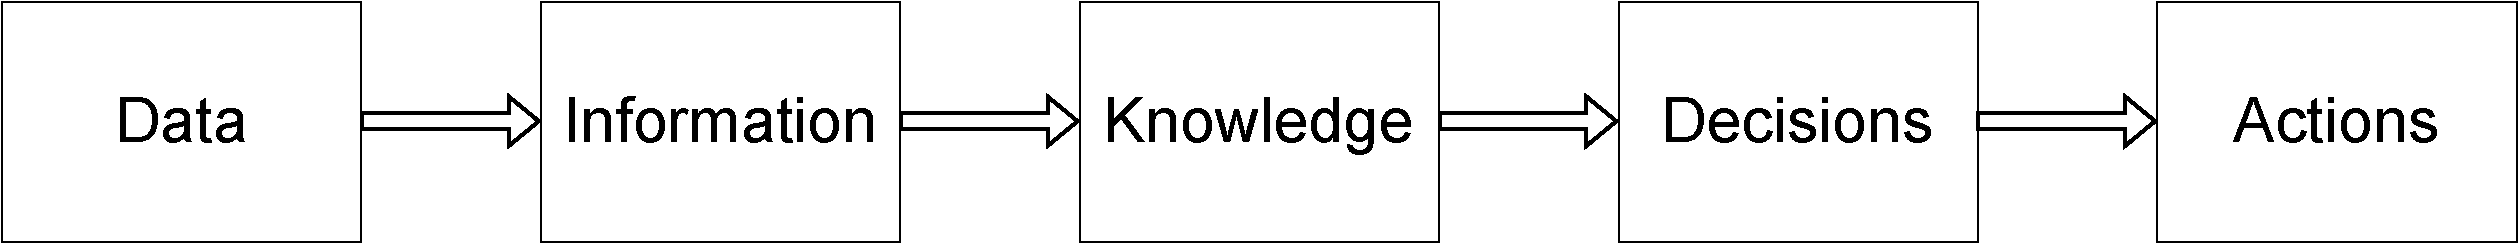
\includegraphics[width=0.99\textwidth, keepaspectratio]{content/02_theretical_foundations/informationValueChain.pdf}
    \caption{Information Value Chain}    
    \label{information_value_chain}
\end{figure}

The information value chain (figure \ref{information_value_chain}) is a set of phases that define the transformation of raw data to information and eventually into knowledge. \enquote{Data} describes raw facts without any structuring. Once organized, the processed data represents \enquote{information}. This \enquote{information} is then used to find patterns and draw conclusions. At this time, the information becomes knowledge \parencite{Fayyad.1996}, \cite{Fayyad.1996b}. This knowledge is then used to make \enquote{decisions} and take corresponding \enquote{actions} \parencite{Sharma.2014}. Each phase of the information value chain also includes a different set of technologies and methodologies. For example, the \enquote{data} phase contains technologies and actions regarding the basic storage of data like database systems or data warehouses \parencite{Abbasi.2016}. The conventional version of this information value chain represents an approach that generally explains the processing of data. The main steps of this information value chain are also applicable for big data \parencite{Abbasi.2016}. This general structure of processing data is also supported by literature from the data analytics field \parencite{Runkler.2020}. In addition, the information value chain contains the further phases \enquote{decisions} and \enquote{actions}, which deal with the influence of the processed data. These phases reflect the impact of data analytics, since data analytics is primarily a technology for the decision-making process \parencite{Runkler.2020}. For this reason, the information value chain is a suitable model to structure different phases in the processing of data in the context of data analytics. %For this reason, the literature examined in this paper is structured according to the phases of the information-value chain.



%\subsection{Boundaries and Conflicts in Organizations}

%This literature review uses the terms boundary and conflict interchangeably. In order to include as much literature as possible, the criteria for boundaries are kept very general. Prior to conducting the literature review, there was no formal definition of boundaries in the context of data analytics used for the selection of literature. Generally, boundaries are described as \enquote{[...] a real or imagined line that marks the limits or edges of something and separates it from other things or places [...]} \parencite{Hornby.2015}. Based on this general description, the term boundary is defined in the context of this elaboration as any circumstance that leads to a reduction in the effectiveness or efficiency of an organization. %Based on this description, the term \enquote{boundary} is defined in the context of this elaboration as any situation that leads to a reduction in the productivity or effectiveness of a company.
%Simultaneously, the term conflict also describes this circumstance. 
%Boundaries and conflicts are therefore used to describe any circumstance that hinders an organization from being perfectly productive. An example of such boundaries or conflicts would be communication issues between different departments, which lead to a reduction of productivity.



%\begin{enumerate}
    %\item \textbf{\textit{Identification of the Problem}}: In this phase, the problem fundamentally solved by the resulting artifact is described. At the same time the value of resulting solution is justified. %The problem identification in this thesis is realized through a literature search which focusses on boundaires and conflicts that limit the utilization of data analyitics.
    %\item \textbf{\textit{Definition of Objectives for a solution}}: This phase focuses on the specific goal of the solution and how its solving can be measured. The objectives for the solution can usually be divided into qualitative and quantitative characteristics. 
    %\item \textbf{\textit{Design and Dev of artefacts}}: This step covers the specific functional design and scope of the artifact and how it is to be achieved. The phase covers both the conceptual design and the specific practical implementation of the solution.
    %\item \textbf{\textit{Demonstration of the Artifact}}: The focus of this phase is to demonstrate that the artifact implemented in the previous step can actually solve the initial problem. For this purpose, various methods such as experiments, case studies or other test setups can be used.
    %\item \textbf{\textit{Evaluation of the solution}}: This step evaluates the artifact and measures how well it contributes to a solution to the problem, therefore this phase tests whether the developed artefact is a valid solution to the research problem. If the artifact does not meet the corresponding requirements, the process is iterated back to step number three. If the artifact meets all requirements and contributes significantly to the solution of the problem, the last step is conducted. 
    %\item \textbf{\textit{Communication}}: The last step ensures that the developed artefact and its value is communicated to the scientific community. The goal of this phase can be achieved through a number of different ways. The choice for the right way of communicating the results thereby relies on the specific topic and problem at hand.
%\end{enumerate}



%The first step, \textit{Identification of the Problem}, \enquote{Define the specific research problem and justify the value of a solution.} (\cite{Peffers.2006}). The 

%Peffers et al. define the phases of the \ac{dsr} methodological in their 2006 article in order  

%\cite{Fulcher.1996}


%Herbert.1996


%Originally conceived in the book \enquote{The Sciences of the Artificial} by Herbert Simon, the research approach of design science research centers primarily on the development of artifacts to solve  theoretical research problems (\cite{Dresch.2004}). 


%"The result of design-science research in IS is, by definition, a purposeful IT artifact created to address an important organizational problem. It must be described effectively, enabling its simple mentation and application in an appropriate domain." \cite{Henver.2004}




%The scientific research process consists in large parts of the formulation of hypothesis and the testing of these hypotheses. The aim of tests being to make statements about a particular object (e.g. a person or a group of persons). These tests are usually conducted using sub-areas (also called characteristics) instead of testing the whole area (\cite{Gniewosz.2011}). One possible way of conducting tests are experiments.

%\section{Artefact Conceptualization Analysis}
%\subsection{Identification of the Problem}
%\subsection{Definition of Objectives for a Solution}
%\subsubsection{Requirement Elicitation}
%\subsubsubsection{Existing Resources for online Epxeriments} 
%\subsubsubsection{Studies in Data Analytics}
%\subsubsection{Requirement Specification}
%\subsubsection{Requirement Validation}
%\subsection{Design and Development of the Artefact}
%\subsubsection{Process Conceptualization}
%\subsubsection{Technology Selection}
%\subsubsubsection{Java}
%\subsubsubsection{Android Studio}
%\subsubsection{System Architecture Development}
%\subsubsubsection{Data Layer}
%\subsubsubsection{Domain Layer}
%\subsubsubsection{user Interface layer}
%\subsubsection{Consolidated System Architecture Summary}
